\section{Results} Several experiments were performed using the evaluation
function mentioned in section \ref{sec:evaluation}. 

Initially the experiments were carried out without the interactive term, $I$,
and without regard for the mass of the individuals produced by the EC. This
meant that the physical part of the evaluation, where Ethan was dropped on the
individuals, resulted in the terms, $E_\Delta$, $E_{rest}$, and $E_{posture}$
all being roughly equivalent between individuals. This happened because the 
higher mass of Ethan would always result in the individuals being rotated and 
Ethan dropping on the floor. This left only the $|V|$ and $R_c$ terms, and the 
EC ultimately optimized towards a minimal voxel count which would not rotate 
when Ethan was dropped, see figure~\ref{fig:flat_object}.

\begin{figure}[ht]
\centering
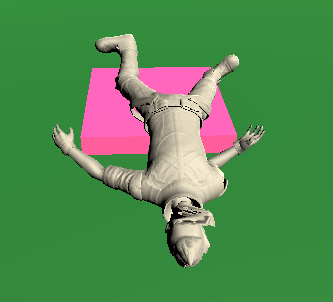
\includegraphics[scale=.5]{flat_chair}
\caption{The evolved object, pink, is simply a flat structure, such that
it does not rotate when Ethan is dropped on it, and has minimal voxel
count.} \label{fig:flat_object} \end{figure}

Adding the interactive term, $I$, did not improve significantly on the above
results. While the selected individual would persist through several
generations, the other best performing individuals would still optimize towards
the aforementioned flat structure, see figure~\ref{fig:selection}.
\begin{figure}[ht]
	\centering
	\subfloat[]{
		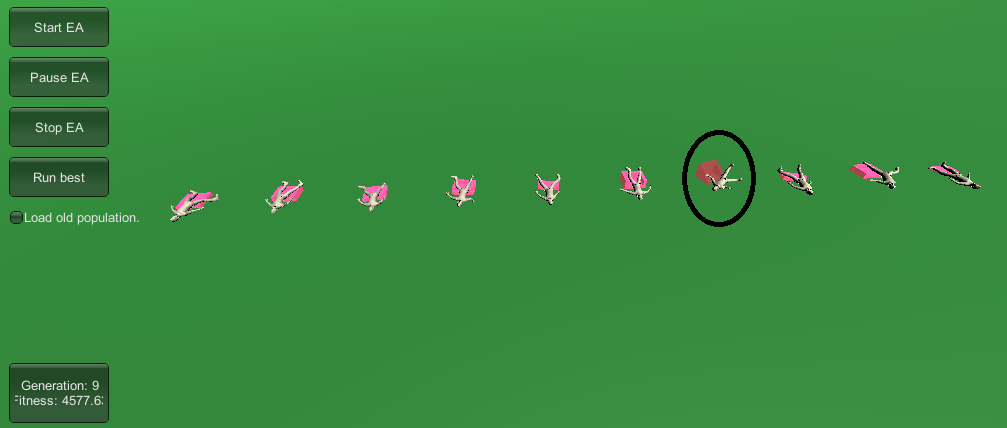
\includegraphics[width=.9\columnwidth, trim={110 0 0 0}, clip]{selection}
	} \hfil
	\subfloat[]{
		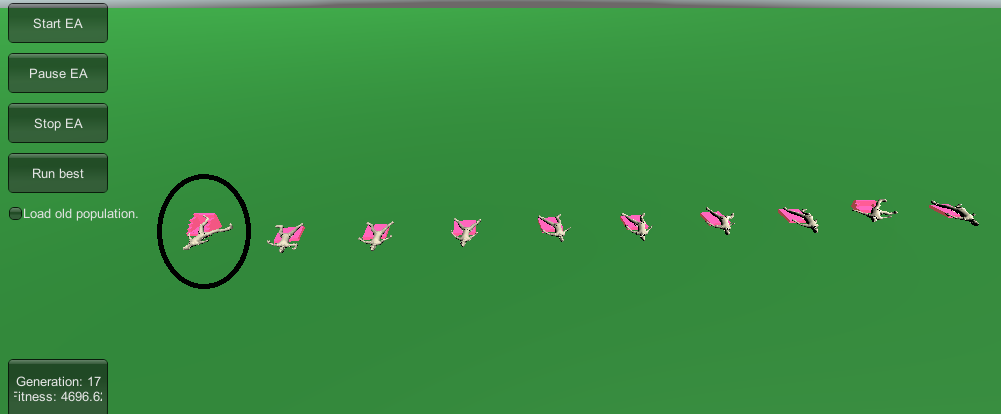
\includegraphics[width=.9\columnwidth, trim={110 0 0 0}, clip]{selection2}
	}
	\caption{Example showing how the selected individual, encircled in (a),
	persists 8 generations later, encircled in (b).} \label{fig:selection}
\end{figure}

Further experiments were conducted, where the mass of the individuals was
adjusted according to their voxel count. In these experiments the EC ended up
producing some individuals which were not just flat objects. Rather it produced
individuals as boxes on which Ethan could rest in a height such that the terms
$E_{rest}$ and $E_\Delta$ were minimized, see figure~\ref{fig:boxchair}.

\begin{figure}[ht]
	\centering
	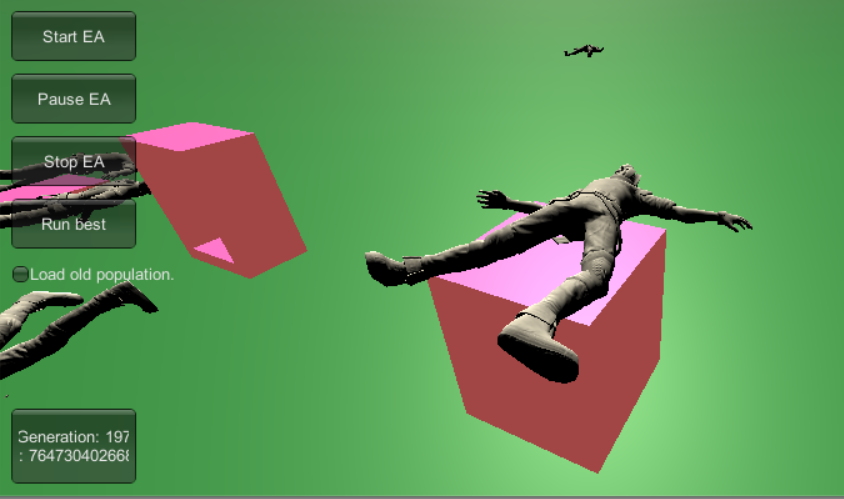
\includegraphics[width=.9\columnwidth, trim={110 0 0 0}, clip]{box_chair}
	\caption{When considering the mass of the individuals, such that more
	compact individuals are more sturdy, the EC evolved a box upon which
	Ethan could rest.}
	\label{fig:boxchair}
\end{figure}
